\subsection{Event Generation}\label{sec:NEUTRINO_GENERATION}
The simulation of low-energy neutrino interactions in \gls{dune} relies on a comprehensive workflow that encompasses several stages, from the event generation to the final analysis data. The workflow is designed to produce realistic simulations of neutrino interactions, accounting for the complex physics processes involved and the detector response. The main stages of the simulation workflow are illustrated in~\cref{fig:SIM_WORKFLOW} and include:

\begin{figure}[ht!]
    \centering
    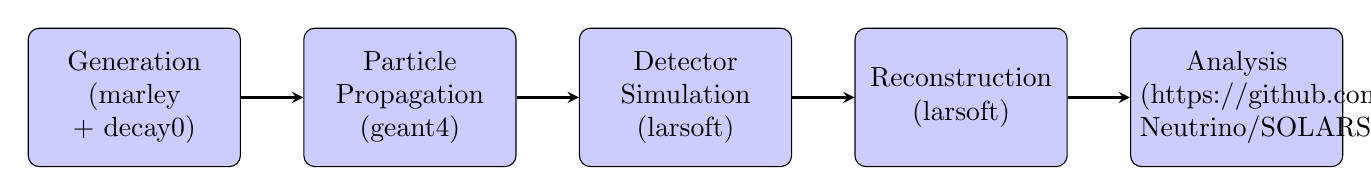
\begin{tikzpicture}[
        node distance=3.5cm,
        block/.style={rectangle, draw, fill=blue!20, text width=7em, text centered, rounded corners, minimum height=5em},
        arrow/.style={thick,->,>=stealth}
    ]
        % Nodes
        \node[block] (gen) {Generation (\gls{marley} + \gls{decay0})};
        \node[block, right of=gen] (prop) {Particle Propagation (\acrshort{geant4})};
        \node[block, right of=prop] (det) {Detector Simulation (\gls{larsoft})};
        \node[block, right of=det] (reco) {Reconstruction (\gls{larsoft})};
        \node[block, right of=reco] (ana) {Analysis (\href{https://github.com/CIEMAT-Neutrino/SOLAR}{SOLAR})};
        
        % Arrows connecting nodes
        \draw[arrow] (gen) -- (prop);
        \draw[arrow] (prop) -- (det);
        \draw[arrow] (det) -- (reco);
        \draw[arrow] (reco) -- (ana);
    \end{tikzpicture}
    \caption{Simulation workflow stages for neutrino event reconstruction in \gls{dune}. The pipeline progresses from event generation through particle propagation, detector simulation, and reconstruction to final analysis.\label{fig:SIM_WORKFLOW}}
\end{figure}

\subsubsection{Neutrino Interactions\label{sec:NEUTRINO_INTERACTIONS}}
The first step in simulating neutrino interactions relies on a comprehensive nuclear model of the possible processes. For low-energy events, this is the \gls{marley}, an event generator developed to simulate the nuclear interactions of low-energy neutrinos in the range of a few to tens of~\unit{\mega\electronvolt}. It is particularly suited for simulating interactions relevant to solar and supernova neutrinos in \gls{lar} detectors. In this work we focus on the \gls{cc} process (although \gls{es} and \gls{nc} have also been implemented):

\begin{equation}
    \nu_e + {}^{40}\mathrm{Ar} \rightarrow e^- + {}^{40}\mathrm{K}^*
\end{equation}

Upon an electron neutrino capture on an argon nucleus and subsequent electron release, the excitation of the residual \( {}^{40}\mathrm{K}^* \) leads to the emission of de-excitation \(\gamma\)-rays, which can produce observable signals (blips) in the vicinity (\SI{<1}{\meter}) of the main electron track (see \cref{fig:EVENT_EDEP}). \gls{marley} incorporates a gamma-decay schemes to describe these processes and feeds the resulting daughter particles into \gls{larsoft}, which is used to produce a \gls{mc} input for physics studies. It simulates primary interaction kinematics, the resulting nuclear state and the gamma-cascades from nuclear de-excitation, as well as, other secondary processes (such as neutron or proton emission). In \gls{dune}'s physics analyses, the most important signature from these interactions is the already mentioned primary electron track. The resulting energy of these is strongly dependent on the de-excitation scheme of the residual nuclear state (see \cref{fig:MARLEY_CC_INTERACTION}). 

\begin{figure}[ht!]
    \centering
    \includegraphics[width=.49\linewidth]{Images/Reco/neutrino_cc_fraction_hd_1x2x6_marley_official_signalparticlek_tsignalsumk_pdg_scan.png}
    \includegraphics[width=.49\linewidth]{Images/Reco/neutrino_cc_production_hd_1x2x6_marley_official_signalparticlek_energy_particle_electron_logz_hist2d.png}
    \caption{\gls{marley}'s computation of \gls{cc} neutrino interaction. (left) Daughter fraction of the original kinetic energy. (Right) Neutrino-electron energy correlation in a CC interaction as predicted by MARLEY.\label{fig:MARLEY_CC_INTERACTION}}
\end{figure}

The average energy transfer and binding energy of the \gls{cc} interaction are displayed. One can observe how the gamma channel starts dominating the interaction up to \SI{\sim 10}{\mega\electronvolt}, and above that threshold, the main electron takes over the fractional energy. This trend is accompanied by a continuous increase in average kinematic threshold caused by the production of additional secondary particles. The most concerning secondary production, from the experimental point of view, is the emission of neutrons; which happens above \SI{\sim15}{\mega\electronvolt}, and leads to a decrease in visible energy that is unlikely to be recovered under realistic reconstruction scenarios. All of these effects combine to a strong energy dependence of the deposited and visible energies, which should be taken into account in our signal calibration. The same can be said about the missing energy due to nuclear binding energy losses, which are also energy dependent and lead to a non-negligible bias in the reconstructed neutrino energy if not properly accounted for. This is particularly important at higher energies, where the binding energy losses can represent a significant fraction of the total neutrino energy.

It is important to mention at this point that a typical low-energy \gls{mc} production includes a full propagation of the backgrounds described in~\cref{sec:BACKGROUND_MODEL}. These additional particles are produced in their specific rates and concentrations according to computations out of the scope of this publication. All particle kinematics and detector placement happen in the so-called \emph{gen} stage of the simulation. All produced background particles follow the same workflow chain as the signal particles and contribute to the ultimate smearing and resolution of the reconstructed objects. In order to account for all possible matching issues one full drift-time needs to be simulated before the neutrino makes its interaction (at $t=0$). After this, the simulation last for another full drift-time to allow neutrinos from all regions of the detector to drift and be collected onto the corresponding readout plane. For the purpose of this publication, neutrinos are produced with isotropic positions and directions across the full active volume; and with a flat energy spectrum from \SI{4}{\mega\electronvolt} up to \SI{30}{\mega\electronvolt}.

\subsubsection{Background Model\label{sec:BACKGROUND_MODEL}}
One of the most studied backgrounds for \gls{lar} detectors is Radon (\(^{222}\text{Rn}\)), which is a noble gas produced in the decay chain of \(^{238}\text{U}\)~\cite{nndc_rn222,borexino_radon,MICROBOONE_RADON_2022}. As a gas, it can diffuse into the active volume of \gls{lar} detectors, where its decay daughters accumulate on surfaces or remain suspended, emitting beta, gamma and alpha radiation (see Appendix~\cref{sec:APPENDIX}). Alpha particles have a very short range in \gls{lar}, but due to their high energy and quenching, they produce significant light signals in the detector, which can be misidentified as low-energy neutrino interaction candidates.

The measurement of low-energy neutrinos in \gls{dune}, particularly those from the Solar \( ^8\mathrm{B} \) chain (\SI{<19}{\mega\electronvolt}), requires a thorough understanding of intrinsic (emitted from the \gls{lar}), component-induced (emanating from detector components) and external (penetrating from the cavern) backgrounds. Understanding the contributions from these particles and decaying isotopes is crucial in achieving a correct vertex and energy reconstruction required for low-energy neutrino analyses. Apart from the previously mentioned radon chain, a comprehensive list of background sources has been implemented in \gls{dune}'s simulation. Presenting \gls{dune}'s full background model is out of the scope of this work. Hence, we focus on providing a brief summary while discussing the features that have the biggest impact on the low-energy neutrino reconstruction analyses.

\begin{itemize}
  \item\textbf{External Backgrounds}: External radiation originates outside the detector's cryostat. The flux is divided into two kinds of particles that manage to penetrate into the detector:

        \begin{itemize}
          \item\textbf{Cavern Neutrons}: Produced by (\(\alpha,n\)) reactions in surrounding rock or via cosmic-ray spallation, neutrons are emitted up to \SI{\sim 10}{\mega\electronvolt} in kinetic energy. They can enter the active volume where they undergo \gls{es} until they capture producing a gamma-cascade which can mimic the topology of a \gls{cc} neutrino interaction. Some neutrons can be captured on the cryostat and other detector components contributing to the environmental particle flux with high energy gammas.
          \item\textbf{Environmental gammas}: High-energy photons from the rock or shotcrete surrounding the detector, typically originating from natural radioactivity. The highest rate contributor to this flux in \gls{dune}'s caver at \gls{surf} is the shotcrete covering the walls. Low-energy gammas (\SI{< 2.7}{\mega\electronvolt}) entering the active volume have a huge flux contributing mostly to worsen the signal reconstruction by mimicking the de-excitation gammas of the \gls{cc} interaction or making the topological distinction between \gls{es} and \gls{cc} less reliable. The higher energy external gammas (\num{2.7} $<$ E \SI{< 14}{\mega\electronvolt}), are produced by \(\gamma\)-decay of isotopes like \(^{208}\text{Tl}\) (\SI{\sim 3.5}{\mega\electronvolt}) or \(^{214}\text{Bi}\) (\SI{\sim 3.27}{\mega\electronvolt}) and secondary nuclear reactions of $(n,\gamma)$ interactions in certain geological environments (\SI{> 6}{\mega\electronvolt}). These high-energy gamma rays are highly site-specific, depending on the local neutron flux and rock composition. Therefore, in situ measurements are fundamental to assess their impact and model accurately their contribution as fake signals to the different physics analyses.
          % \item \textbf{Cosmic rays}: Even in underground environments, muons and cosmogenically produced secondaries can lead to spallation products and radiogenic activation of detector materials.
        \end{itemize}

  \item \textbf{Component-Induced Backgrounds}: These can arise from the materials used to construct the detector itself. Material screening and selection, as well as radon mitigation systems, are essential to reduce these sources. These include decay chains of long-lived isotopes introduced during fabrication or operation. Some of the most prominent are:

        \begin{itemize}
          \item \textbf{Uranium (\(^{238}\)U)}: Produces alpha, beta, and gamma emissions, as well as daughters like \(^{214}\)Bi and \(^{210}\)Pb.
          \item \textbf{Thorium (\(^{232}\)Th)}: Similar to the uranium chain, with prominent gamma emitters like \(^{208}\)Tl (\SI{2.6}{\mega\electronvolt}).
          \item \textbf{Potassium (\(^{40}\)K)}: Often present in plastics and glass (like the ones used for traditional photon detectors). It emits a \SI{1.46}{\mega\electronvolt} gamma line.
          \item \textbf{Radon (\(^{222}\)Rn)}: Present in atmospheric air and therefore very difficult to prevent from accumulation on detector and component surfaces during construction.
        \end{itemize}

  \item \textbf{Intrinsic Liquid Argon Backgrounds}: When talking about the properties of \gls{dune}'s \gls{lar} we are generalizing the properties of (\(^{40}\)Ar) but certain radioactive isotopes are either present naturally in atmospheric argon or may be introduced as impurities:

        \begin{itemize}
          \item \textbf{Argon (\(^{39}\)Ar)}: A beta emitter with an endpoint energy of \SI{565}{\kilo\electronvolt} and a half-life of 269 years. It dominates the low-energy spectrum in atmospheric argon with an activity of \SI{\sim1}{\becquerel\per\kilo\gram}. Together with the external gammas, this background contributes to the smearing of signals and worsens the hit reconstruction efficiency of the \gls{tpc} by significantly altering the waveforms and providing fake signal candidates for plane-matching.
          \item \textbf{Argon (\(^{42}\)Ar) and Potassium (\(^{42}\)K)}: Rare isotopes that decay via beta emission. \(^{42}\)K emits an electron (\(Q \sim 3.5\)\unit{\mega\electronvolt}), which is particularly problematic due to its similarity to low-energy solar neutrino events.
          \item \textbf{Krypton (\(^{85}\)Kr)}: A beta emitter with a \(Q\)-value of \SI{687}{\kilo\electronvolt}, introduced via contamination from air or during purification. Often requires cryogenic distillation to remove. It contributes to the low-energy background spectrum, similar to \(^{39}\)Ar.
          \item \textbf{Radon (\(^{222}\)Rn)}: In addition to emanation from components, radon can dissolve in liquid argon and contribute to intrinsic backgrounds through its decay chain that can appear throughout the full \gls{lar} volume.
        \end{itemize}
\end{itemize}

\begin{figure}[ht!]
    \centering
    \includegraphics[width=.49\linewidth]{Images/LowE/background_hd_1x2x6_centralapa_energy_counts_ar39_kr85_ar42_rn22x_cpa_apa_gamma_neutron_logy_scan.png}
    \includegraphics[width=.49\linewidth]{Images/LowE/background_hd_1x2x6_centralapa_energy_counts_electron_gamma_alpha_neutron_logy_scan.png}
  \caption{Simulated particle flux from \gls{dune}'s Background Model version 3. (Left) Divided by the background component. (Right) Divided by particle type. The external gamma and neutron flux are computed for the inner surfaces of the cryostat, where they are further propagated and combined with the rest of the intrinsic backgrounds.\label{fig:BACKGROUND_MODEL}}
\end{figure}
%The relative importance of these isotopes depends on the source of argon: underground argon (UAr) has significantly reduced \(^{39}\)Ar activity compared to atmospheric argon (AAr).
In \gls{dune}, \gls{lar} purification and recirculation installations are planned to ensure constant operating conditions. A detailed background model informed by in situ measurements, simulations, and radiopurity assays has been developed and is under constant revision to ensure accurate predictions of the background fluxes in the \gls{lar} active volume. The model is implemented in the \gls{larsoft}~\cite{LARSOFT}, the software framework used for \gls{dune}'s simulations, and is used to generate realistic event samples for detector response studies and physics analyses. \Cref{fig:BACKGROUND_MODEL}, shows the latest simulated particle flux from the background model (v. 3.6) on top of the predicted solar spectrum as a function of the particles' kinetic energy. The left panel shows the flux divided by background components, while the right panel shows it divided by particle type. The flux is dominated by external gammas, argon and krypton at low- and external gammas and neutrons at high-energies. These figures highlight the importance of understanding these backgrounds by highlighting the huge difference in flux between the low-energy neutrino signal and the background components. Without a proper energy calibration, the smearing of the background components can lead to a significant loss of signal efficiency and a degradation of the energy resolution.